\documentclass[openany]{book}
\input{notes_white}
\usepackage{mathtools}
\usepackage{pgfplots}
\usepackage{chemfig}
\settitle{Biology Lab - Enzyme Kinetics}
\begin{document}
\title{\Large{\underemphasise{Enzyme Kinetics}} \\ \vspace{5pt}
\large{To study the enzyme kinetics of the enzyme alkaline phosphatase}}
\author{Eklavya Raman \\ \vspace{5pt} er24ms024@iiserkol.ac.in \\ \vspace{5pt}}
\date{\today}
\maketitle
\begin{center}
    \textbf{Abstract}
\end{center}
    Enzyme kinetics is the study of the rates of enzymatic reactions and how they are influenced by various factors such as substrate concentration, enzyme concentration, temperature, and pH. In this experiment, we will investigate the kinetics of the enzyme alkaline phosphatase (ALP) using p-nitrophenyl phosphate (pNPP) as a substrate. 
\subsubsection{Principle and Working Formulae}
Alkaline phosphatase catalyzes the hydrolysis of p-nitrophenyl phosphate (pNPP) to produce p-nitrophen -ol (pNP) and inorganic phosphate. The reaction can be monitored by measuring the increase in absorbance at 405 nm due to the formation of p-nitrophenol, which is yellow in color under alkaline conditions. By varying the substrate concentration and measuring the initial reaction rates, we can determine key kinetic parameters such as the Michaelis-Menten constant (Km) and maximum velocity (Vmax) of the enzyme. \\ 
Let specific activity ($SA$) be defined as the amount of product formed per unit time per mg of enzyme ($\mu \text{mol min}^{-1} \text{mg}^{-1}$). We have - 
$$SA = \frac{V (\mu \text{mol min}^{-1}) \times \text{Reaction Volume (mL)}}{\text{Amount of Enzyme (mg)}}$$
Where, V is the velocity of the reaction.
We can calculate the velocity using the Michaelis-Menten curve. The Michaelis-Menten equation is given by:
$$V = \frac{V_{max} [S]}{K_m + [S]}$$
Where,
\begin{itemize}
    \item $V$ = Initial reaction velocity
    \item $V_{max}$ = Maximum reaction velocity
    \item $[S]$ = Substrate concentration
    \item $K_m$ = Michaelis-Menten constant
\end{itemize}
By plotting the initial reaction velocities against substrate concentrations, we can fit the data to the Michaelis-Menten equation to determine $K_m$ and $V_{max}$.
We can calculate the velocities by estimating the amount of pNP formed over time. The concentration of pNP can be determined by plotting a standard curve of absorbance at 405 nm against known concentrations of pNP. Using the standard curve, we can convert the absorbance values obtained from the reaction mixture to pNP concentrations. The initial reaction velocity (V) can then be calculated as the change in pNP concentration over time.
\subsubsection{Reaction}
\begin{figure}[H]
    \centering
    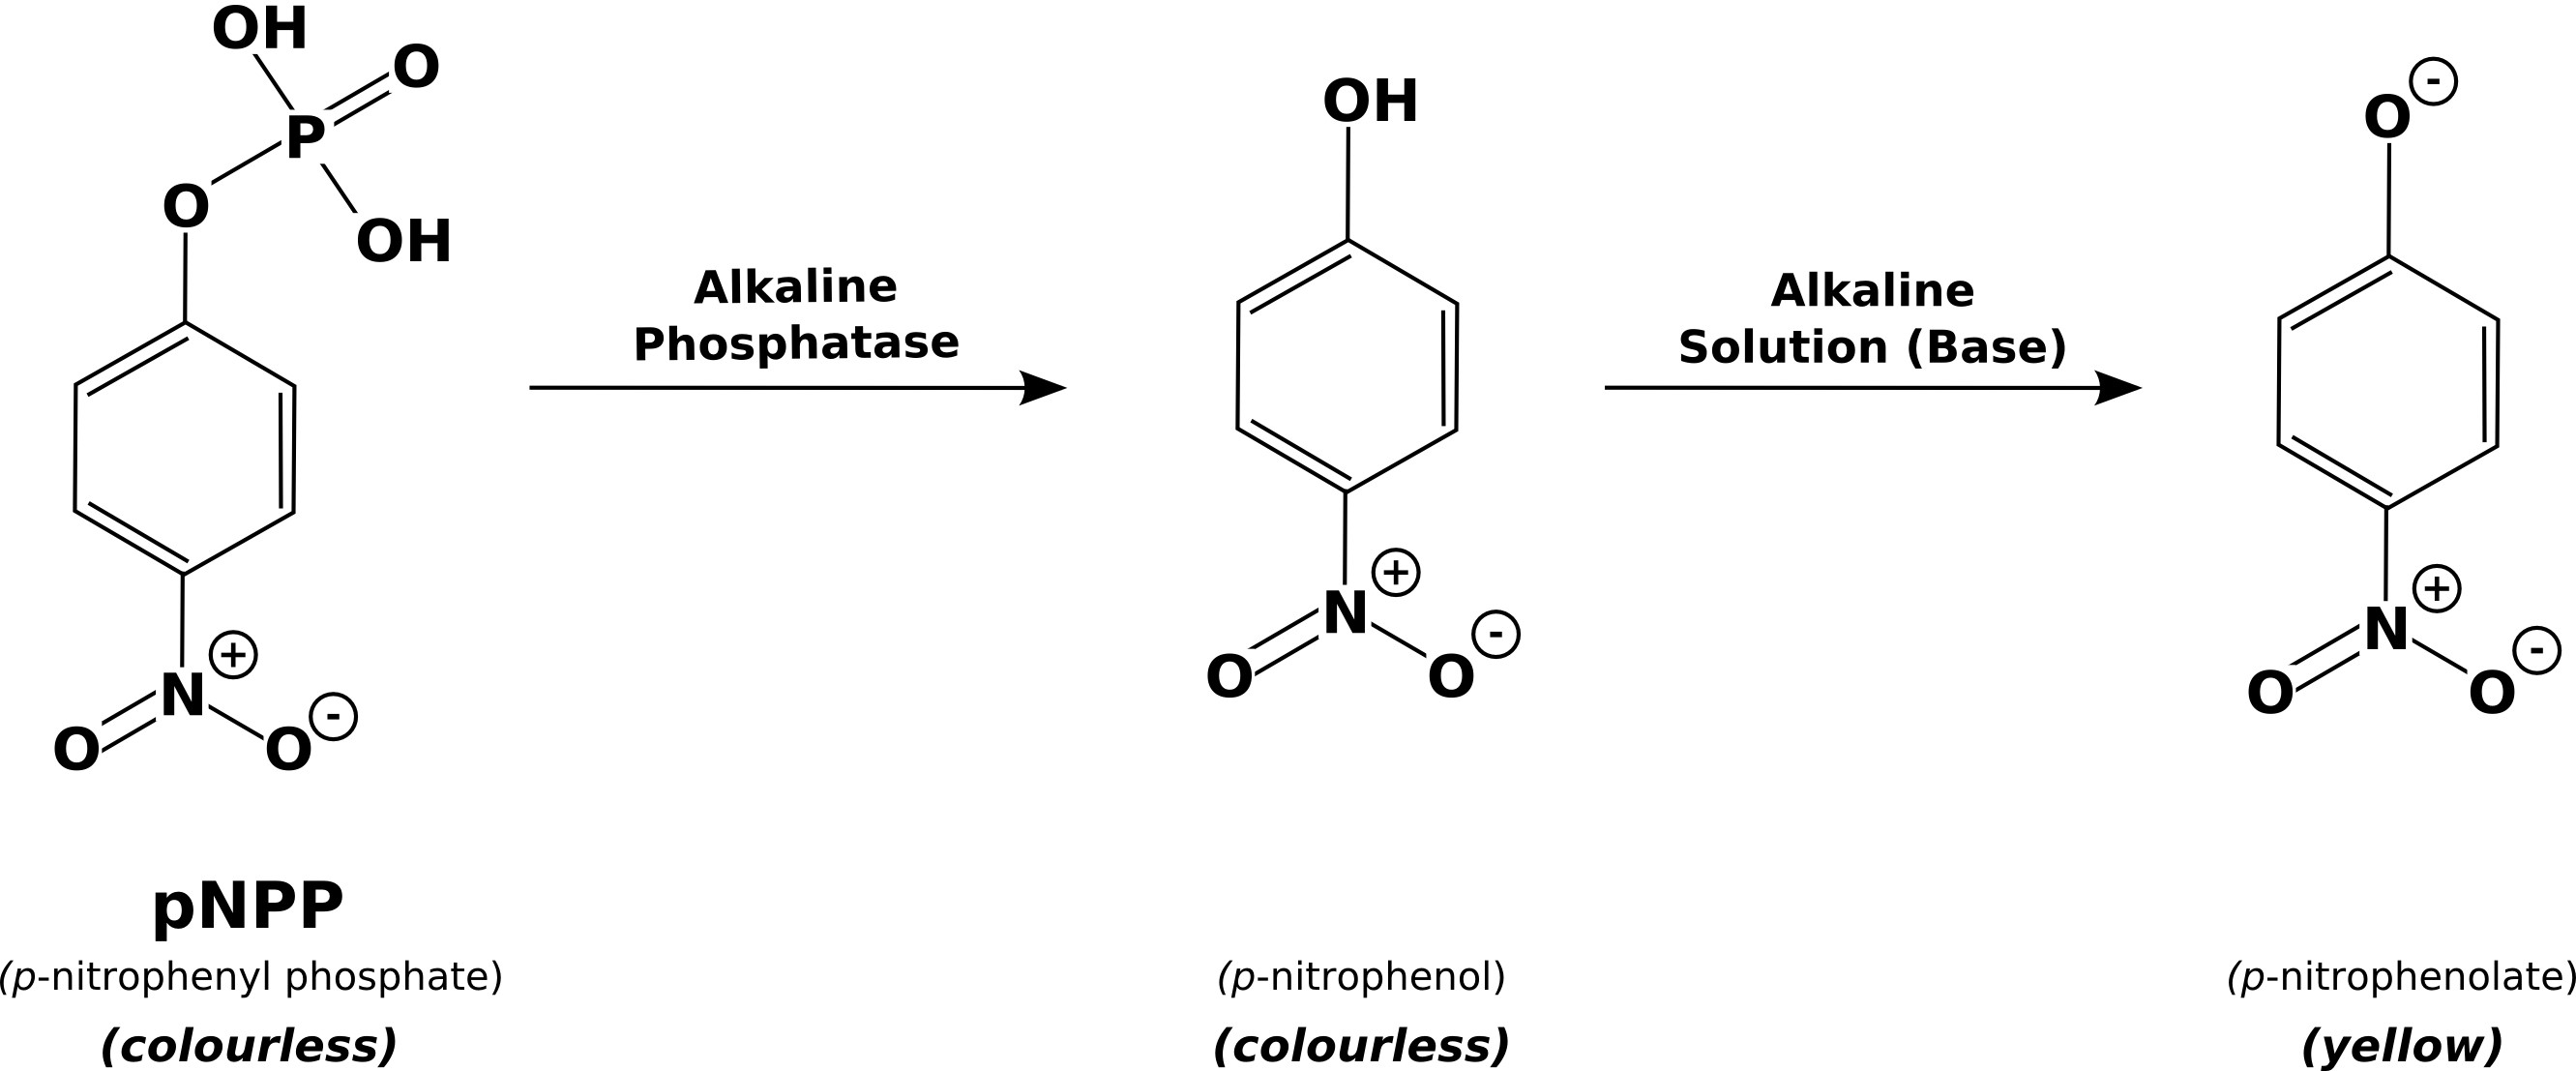
\includegraphics[width=0.8\textwidth]{images/seap-kit-results.jpg}
    \caption{Hydrolysis of pNPP by Alkaline Phosphatase}
    \label{fig:reaction}
\end{figure}
Trans Acetylation of pNPP by ALP to form pNP and inorganic phosphate. We use NAOH and buffer to maintain alkaline pH for the reaction to proceed optimally. 
\subsubsection{Observations and Results}
The standard curve for p-nitrophenol (pNP) was generated by measuring the absorbance of known concentrations of pNP at 405 nm. The following table summarizes the data collected for the standard curve:
\begin{table}[H]
\centering
\renewcommand{\arraystretch}{1.3}
\resizebox{\textwidth}{!}{
\begin{tabular}{|
    c
  | c
  | c
  | c
  | c
  | c
  | c
|}
\hline
\textbf{Reaction Tubes} &
\textbf{Volume of Buffer (µL)} &
\textbf{Vol. of 200 µM pNP (µL)} &
\textbf{Volume of 1N NaOH} &
\textbf{pNP Concentration (µM)} &
\textbf{Absorbance} &
\textbf{Avg.} \\
\hline

Blank & 1000 & 0 & 1 mL & 0 & 0 &  \\ \hline
Blank & 1000 & 0 & 1 mL & 0 & 0 &  \\ \hline

1 & 985 & 15 & 1 mL & 3 & 0.006 & 0.005 \\ \hline
1 (dup) & 985 & 15 & 1 mL & 3 & 0.004 & 0.005 \\ \hline

2 & 975 & 25 & 1 mL & 5 & 0.010 & 0.0095 \\ \hline
2 (dup) & 975 & 25 & 1 mL & 5 & 0.009 & 0.0095 \\ \hline

3 & 950 & 50 & 1 mL & 10 & 0.023 & 0.024 \\ \hline
3 (dup) & 950 & 50 & 1 mL & 10 & 0.025 & 0.024 \\ \hline

4 & 925 & 75 & 1 mL & 15 & 0.046 & 0.046 \\ \hline
4 (dup) & 925 & 75 & 1 mL & 15 & 0.046 & 0.046 \\ \hline

5 & 900 & 100 & 1 mL & 20 & 0.057 & 0.0585 \\ \hline
5 (dup) & 900 & 100 & 1 mL & 20 & 0.060 & 0.0585 \\ \hline

6 & 875 & 125 & 1 mL & 25 & 0.075 & 0.0775 \\ \hline
6 (dup) & 875 & 125 & 1 mL & 25 & 0.080 & 0.0775 \\ \hline

7 & 850 & 150 & 1 mL & 30 & 0.090 & 0.098 \\ \hline
7 (dup) & 850 & 150 & 1 mL & 30 & 0.098 & 0.098 \\ \hline

8 & 800 & 200 & 1 mL & 40 & 0.128 & 0.130 \\ \hline
8 (dup) & 800 & 200 & 1 mL & 40 & 0.132 & 0.130 \\ \hline

\end{tabular}
} % end resizebox
\caption{Standard Curve Data for p-Nitrophenol (pNP)}
\end{table}
Using the above data, we plot a standard curve of Absorbance vs pNP Concentration to determine the concentration of pNP formed in the reaction mixtures. \\
\begin{figure}[H]
    \centering
    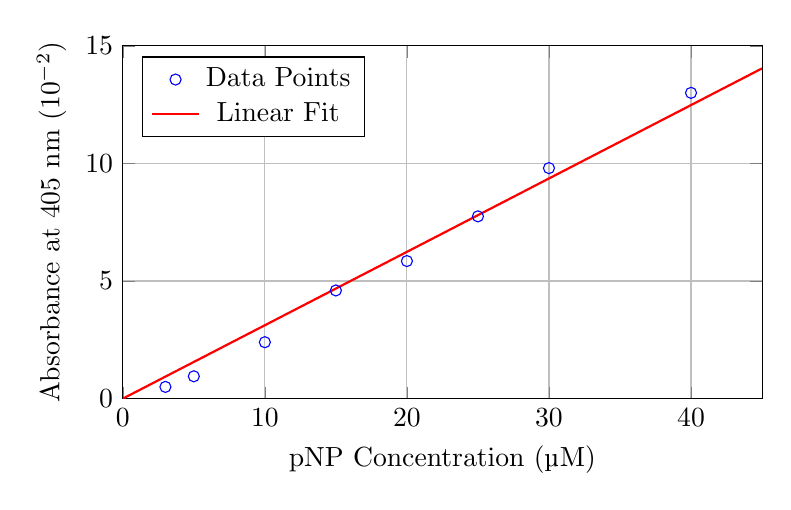
\begin{tikzpicture}
        \begin{axis}[
            width=0.8\textwidth,
            height=0.5\textwidth,
            xlabel={pNP Concentration (µM)},
            ylabel={Absorbance at 405 nm ($10^{-2}$)},
            grid=major,
            xmin=0, xmax=45,
            ymin=0, ymax=15,
            domain=0:45,
            samples=100,
            legend pos=north west,
        ]
        % Plot data points
        \addplot[only marks, mark=o, blue] coordinates {
            (3, 0.5)
            (5, 0.95)
            (10, 2.4)
            (15, 4.6)
            (20, 5.85)
            (25, 7.75)
            (30, 9.8)
            (40, 13.0)
        };
        \addlegendentry{Data Points}

        % Plot linear fit
        \addplot[red, thick] {0.312*x + 0.0005};
        \addlegendentry{Linear Fit}
        \end{axis}
    \end{tikzpicture}
    \caption{Standard Curve of p-Nitrophenol (pNP)}
    \label{fig:standard_curve}
\end{figure}
We have the linear fit equation as -
$$\text{Absorbance} = 0.00345 \times \text{pNP Concentration (µM)} + 0.0005$$
Next, we measure the absorbance values for different substrate concentrations in the presence of alkaline phosphatase enzyme. Using this data, we can calculate the amount of pNP formed and subsequently the initial reaction velocities. The following table summarizes the values obtained from the enzyme kinetics experiment:
\begin{table}[H]
\centering
\renewcommand{\arraystretch}{1.3}
\resizebox{\textwidth}{!}{
\begin{tabular}{|
    p{1.8cm}  % Reaction tube
  | p{1.8cm}  % [S]
  | p{1.8cm}  % 1/[S]
  | p{2.2cm}  % Absorbance
  | p{3cm}    % Product formed
  | p{3cm}    % V = P/time
  | p{2cm}    % Avg V
  | p{3cm}    % 1/V
  | p{2cm}    % Avg 1/V
|}
\hline
\textbf{Reaction tubes} &
\textbf{[S] (mM)} &
\textbf{1/[S] (mM\textsuperscript{-1})} &
\textbf{Absorbance - CF} &
\textbf{(P) Product formed from std. curve (µM)} &
\textbf{V = P/time (µM min\textsuperscript{-1})} &
\textbf{Avg.} &
\textbf{1/V (µM\textsuperscript{-1} min)} &
\textbf{Avg.} \\
\hline

% ---- Add rows here ----
1 & 0.1 & 10 & 0.020 & 8.1014 & 0.54 & & 1.85 & \\
\hline
2 & 0.1 & 10 & 0.020 & 8.1014 & 0.54 & 0.54 & 1.85 & 1.85 \\
\hline
3 & 0.25 & 4 & 0.016 & 6.9420 & 0.46 & & 2.17 & \\
\hline
4 & 0.25 & 4 & 0.023 & 8.9710 & 0.59 & 0.52 & 1.69 & 1.93 \\
\hline
5 & 0.5 & 2 & 0.048 & 16.2173 & 1.08 & & 0.93 & \\
\hline
6 & 0.5 & 2 & 0.046 & 15.6376 & 1.04 & 1.06 & 0.96 & 0.94 \\
\hline
7 & 0.75 & 1.33 & 0.048 & 16.2173 & 1.08 & & 0.93 & \\
\hline
8 & 0.75 & 1.33 & 0.039 & 13.6086 & 0.90 & 0.99 & 1.11 & 1.01 \\
\hline
9 & 1 & 1 & 0.057 & 18.8260 & 1.25 & & 0.8 & \\
\hline
10 & 1 & 1 & 0.055 & 18.2463 & 1.21 & 1.23 & 0.83 & 0.82 \\
\hline
11 & 2 & 0.5 & 0.063 & 20.5652 & 1.37 & & 0.72 & \\
\hline
12 & 2 & 0.5 & 0.065 & 21.1449 & 1.40 & 1.39 & 0.71 & 0.72 \\
\hline
13 & 2.5 & 0.4 & 0.064 & 20.8550 & 1.39 & & 0.72 & \\
\hline
14 & 2.5 & 0.4 & 0.066 & 21.4347 & 1.42 & 1.41 & 0.70 & 0.72 \\
\hline
15 & 5.0 & 0.2 & 0.054 & 17.9565 & 1.19 & & 0.84 & \\
\hline
16 & 5.0 & 0.2 & 0.071 & 22.8840 & 1.52 & 1.36 & 0.65 & 0.74 \\
\hline
17 & 7.5 & 0.13 & 0.074 & 23.7536 & 1.58 & & 0.63 & \\
\hline
18 & 7.5 & 0.13 & 0.064 & 20.8550 & 1.39 & 1.49 & 0.72 & 0.67 \\
\hline
19 & 9 & 0.11 & 0.073 & 23.4637 & 1.56 & & 0.64 & \\
\hline
20 & 9 & 0.11 & 0.079 & 25.2028 & 1.68 & 1.62 & 0.59 & 0.62 \\
\hline
\end{tabular}}
\caption{Observations and Results for Enzyme Kinetics of Alkaline Phosphatase}
\end{table}
Now, we can plot the Michaelis-Menten curve to determine the kinetic parameters $K_m$ and $V_{max}$.
\begin{figure}[H]
    \centering
    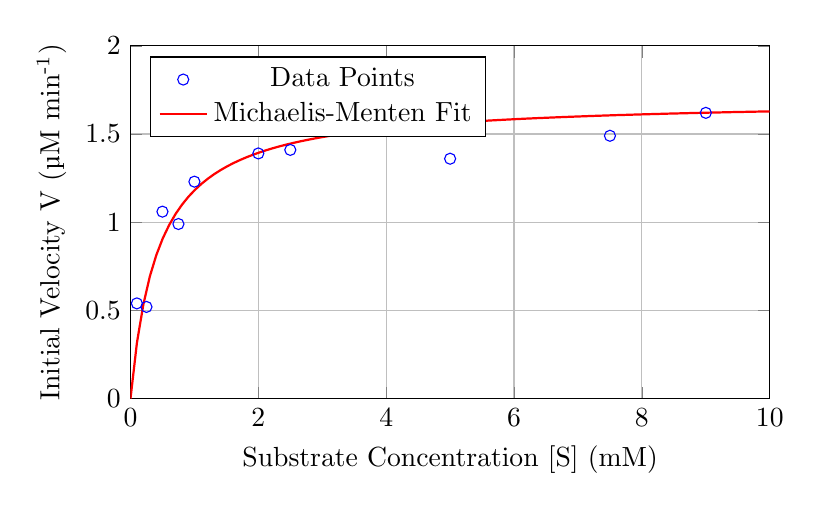
\begin{tikzpicture}
        \begin{axis}[
            width=0.8\textwidth,
            height=0.5\textwidth,
            xlabel={Substrate Concentration [S] (mM)},
            ylabel={Initial Velocity V (µM min\textsuperscript{-1})},
            grid=major,
            xmin=0, xmax=10,
            ymin=0, ymax=2,
            domain=0:10,
            samples=100,
            legend pos=north west,
        ]
        % Plot data points
        \addplot[only marks, mark=o, blue] coordinates {
            (0.1, 0.54)
            (0.25, 0.52)
            (0.5, 1.06)
            (0.75, 0.99)
            (1, 1.23)
            (2, 1.39)
            (2.5, 1.41)
            (5, 1.36)
            (7.5, 1.49)
            (9, 1.62)
        };
        \addlegendentry{Data Points}

        % Plot Michaelis-Menten fit
        \addplot[red, thick] {1.7*x/(0.44 + x)};
        \addlegendentry{Michaelis-Menten Fit}
        \end{axis}
    \end{tikzpicture}
    \caption{Michaelis-Menten Curve for Alkaline Phosphatase}
    \label{fig:michaelis_menten}
\end{figure}
From the Michaelis-Menten curve, we can estimate the kinetic parameters:
\begin{itemize}
    \item $V_{max} \approx 1.7 \, \mu \text{M min}^{-1}$
    \item $K_m \approx 0.44 \, \text{mM}$
\end{itemize}
We can also plot the Lineweaver-Burk plot to confirm these values. The Lineweaver-Burk equation is given by:
$$\frac{1}{V} = \frac{K_m}{V_{max}} \cdot \frac{1}{[S]} + \frac{1}{V_{max}}$$

\begin{figure}[H]
    \centering
    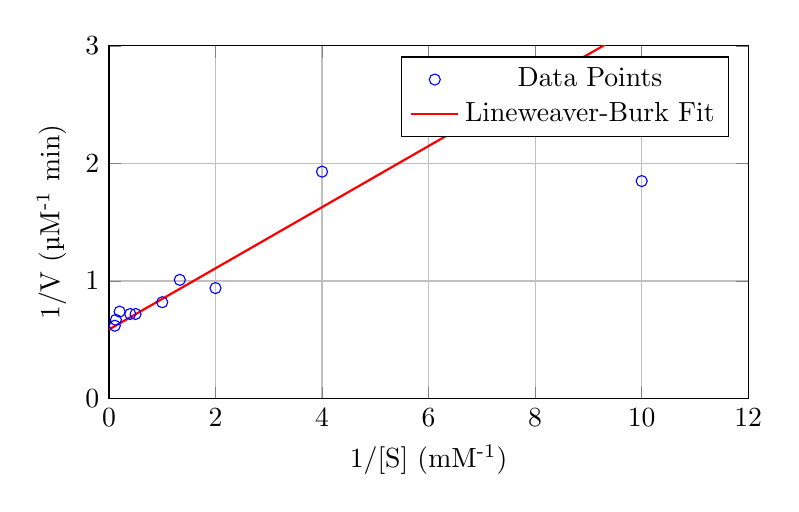
\begin{tikzpicture}
        \begin{axis}[
            width=0.8\textwidth,
            height=0.5\textwidth,
            xlabel={1/[S] (mM\textsuperscript{-1})},
            ylabel={1/V (µM\textsuperscript{-1} min)},
            grid=major,
            xmin=0, xmax=12,
            ymin=0, ymax=3,
            domain=0:12,
            samples=100,
            legend pos=north east,
        ]
        % Plot data points
        \addplot[only marks, mark=o, blue] coordinates {
            (10, 1.85)
            (4, 1.93)
            (2, 0.94)
            (1.33, 1.01)
            (1, 0.82)
            (0.5, 0.72)
            (0.4, 0.72)
            (0.2, 0.74)
            (0.13, 0.67)
            (0.11, 0.62)
        };
        \addlegendentry{Data Points}

        % Plot Lineweaver-Burk fit
        \addplot[red, thick] {0.26*x + 0.588};
        \addlegendentry{Lineweaver-Burk Fit}
        \end{axis}
    \end{tikzpicture}
    \caption{Lineweaver-Burk Plot for Alkaline Phosphatase}
    \label{fig:lineweaver_burk}
\end{figure}
From the Lineweaver-Burk plot, we can confirm the kinetic parameters:
\begin{itemize}
    \item $V_{max} = \frac{1}{\text{y-intercept}} \approx 1.7 \, \mu \text{M min}^{-1}$
    \item $K_m = \text{slope} \times V_{max} \approx 0.44 \, \text{mM}$
\end{itemize}

\subsubsection{Calculations}
Using the determined values of $V_{max}$ and $K_m$, we can calculate the specific activity ($SA$) of the enzyme. Assuming a reaction volume of 1 mL and an enzyme concentration of 0.1 mg, we have:
$$SA = \frac{V_{max} \times \text{Reaction Volume}}{\text{Amount of Enzyme}} = \frac{1.7 \, \mu \text{M min}^{-1} \times 1 \, \text{mL}}{0.1 \, \text{mg}} = 17 \, \mu \text{mol min}^{-1} \text{mg}^{-1}$$
\subsubsection{Conclusion}
In this experiment, we successfully studied the enzyme kinetics of alkaline phosphatase using p-nitrophenyl phosphate as a substrate. We determined the kinetic parameters $K_m$ and $V_{max}$, and calculated the specific activity of the enzyme. The results provide insights into the catalytic efficiency of alkaline phosphatase and its behavior under varying substrate concentrations.
\subsubsection{Discussion and Sources of Error}
Several factors could have influenced the accuracy of our results. Potential sources of error include:
\begin{itemize}
    \item Inaccurate pipetting leading to errors in substrate and enzyme concentrations.
    \item Variability in absorbance measurements due to instrument calibration or cuvette inconsistencies.
    \item Incomplete mixing of reaction components, affecting reaction rates.
    \item Temperature fluctuations during the experiment, impacting enzyme activity.
    \item Assumption of constant enzyme activity over the course of the reaction.
\end{itemize}
Careful attention to experimental protocols and repeated trials can help mitigate these errors in future studies. With further refinement, more precise kinetic parameters can be obtained, enhancing our understanding of alkaline phosphatase's enzymatic behavior.

\end{document}